
\section{Old}

\begin{lemma}[\cite{laracuente_quantum_2025}, Lemma 3.1] \label{lem:chainmin1}
Let $(\Phi_j)_{j=1}^m$ be a given family of quantum channels with respective $(\lambda_j)_{j=1}^m$-SDPI and decoherence-free subspace projections $(\E_j)_{j=1}^m$, $\E$ a joint decoherence-free subspace projection commuting with each $\Phi_j$ (for which $\E \E_j = \E_j \E = \E$),
%\fl{The 'joint' here seems to refer to the fact that $\E_m\circ \E = \E$? You seem to use this when applying the chain rule in \eqref{eq:chain2} below.}
and $(\Psi_j)_{j=1}^m$ a family of channels each commuting with $\E$. Then
%\fl{What are the `rotations' that you're referring to here? Do you mean the $\E_j$?}
\begin{equation*}
    \begin{split}
         D(\rho \| \E(\rho)) - D((\Psi_m \Phi_m) \dots (\Psi_1 \Phi_1) (\rho) \| \E (''))
            \mbnline \mbalign \geq \sum_{j=1}^m \lambda_j D( (\Psi_{j-1} \Phi_{j-1}) \dots (\Psi_1 \Phi_1)(\rho) \| \E_j ('')) \pl,
    \end{split}
\end{equation*}
where when $''$ appears in the second argument to relative entropy, it is equal to the first argument.
\end{lemma}
\begin{prop}[\cite{laracuente_quasi-factorization_2022}, Proposition I.6] \label{prop:decay-merge}
Let $\{\Phi^t_j : j \in 1...J \in \NN\}$ be GNS self-adjoint quantum Markov semigroups such that $\Phi_j^t = \exp(- \L_j t)$ with fixed point conditional expectation $\E_{j} = \lim_{t \rightarrow \infty} \Phi_j^t$ admitting common invariant state $\sigma$. Let $\E_{\sigma *}$ be the weighted intersection fixed point conditional expectation. Let $\Phi^t$ be the semigroup generated by $\L = \sum_j \alpha_j \L_j + \L_0$, where $\L_0$ generates $\Phi_0^t$ such that $\Phi_0^t \E_{\sigma *} = \E_{\sigma *} \Phi_0^t = \E_{\sigma *}$. If the conditional expectations $(\alpha_j)$-quasi-factorize, and each $\Phi^t_j$ has $\lambda$-(C)MLSI, then $\Phi^t$ has $\lambda$-(C)MLSI.
\end{prop}
\begin{lemma}[Chain Rule] \label{lem:chainexp}
Let $\omega$ be a density and $\E$ be a conditional expectation such that $\E(\omega) = \omega$. Then for any density $\rho$,
\begin{equation*}
D(\rho \| \omega) = D(\rho \| \E(\rho)) + D(\E(\rho) \| \omega) \pl.
\end{equation*}
\end{lemma}
Lemma \ref{lem:chainexp} is a well-known identity in quantum information. An important consequence of Lemma \ref{lem:chainexp} is that for any channel $\Phi$ and conditional expectation $\E'$,
\begin{equation} \label{eq:chain-iter}
    D(\rho \|\Psi(\rho)) + D(\rho \| \E'(\rho))
        \geq D(\E'(\rho) \| \E' \circ \Psi(\rho)) + D(\rho \| \E'(\rho))
    = D(\rho \| \E' \circ \Psi(\rho)) \pl.
\end{equation}
\begin{lemma}[\cite{laracuente_quasi-factorization_2022}, Corollary II.15. \cite{gao_complete_2025}, Lemma 2.3]  \label{lem:revconv}
Let $\rho$ be a density and $\E,\Psi$ be quantum channels such that
\begin{equation}
    (1 - \epsilon) \E \prec \Psi(\rho) \prec (1 + \delta) \E
\end{equation}
%\begin{equation}
%    (1-\epsilon) \E(\rho) + \epsilon \Phi(\rho) \leq (1 + \delta) \E(\rho)
%\end{equation}
for constants $\epsilon, \delta \in (0,1)$. Assume $\rho \in \text{supp}(\E(\rho))$. Furthermore, assume $\Psi \E = \E$. Then
\begin{equation}
D(\rho \| \Psi(\rho)) \geq \beta_{\epsilon, \delta} D(\rho \| \E(\rho))
\end{equation}
with
\begin{equation} \label{eq:simpleG} 
    \beta_{\epsilon, \delta} \geq \frac{1}{{(1 + \epsilon)(1 + \delta)}} \Big ( 1 - \frac{2 (1 + \epsilon) \delta^2}{(\epsilon + \delta)(\ln (1 + \delta / \epsilon) - 1) + \epsilon} - 4 \epsilon - \epsilon^2 \Big ) \pl.
\end{equation}
If $\epsilon = \delta$, then
\begin{equation}
    \beta_{\epsilon, \epsilon} \geq \frac{1-\epsilon}{1 + \epsilon} - \frac{\epsilon}{(1 - \epsilon) (2 \ln 2 - 1)} \pl, \text{ and } \beta_{\epsilon, \epsilon} \geq 1 - 12 \epsilon \pl.
\end{equation}
If $\epsilon \leq 1/10$, then $\beta_{\epsilon, \epsilon} \geq 1/2$.
\end{lemma}
\begin{lemma}[Iterated Logarithm Formula from \cite{laracuente_quantum_2025}, New Unpublished Version] \label{lem:log-iterate}
    Consider the function $R(x) = a (\ln x + b)$ for $a, b, x \geq 1$. Let $m = \log^*(x)$, the iterated logarithm with base $e$. Assume $b \geq 3$. Then
    \begin{equation}
        R^m(x) \leq a (b + \ln a) \pl.
    \end{equation}
\end{lemma}
\begin{definition} \label{def:quasifactorization}
    Let $\{\E_j\}_{j=1}^m$ be a set of conditional expectations with the common invariant state $\sigma$ and $\sigma$-weighted intersection subalgebra projection $\E$. We say that the set $(\alpha_j)$-quasi-factorizes (in other texts, has $\alpha$-approximate tensorization) if
    \begin{equation}
        \sum_j \alpha_j D(\cdot \| \E_j(\cdot)) \geq D(\cdot \| \E(\cdot)) \pl.
    \end{equation}
\end{definition}
\begin{assump}[Gluing Assumption] \label{assump:glue} \normalfont
    Let $\E_A$ and $\E_B$ be subspace projections, and $\E$ be the projection to their intersection subspace. If $A$ and $B$ act non-trivially on a joint space with $m$ elementary units, then $\E_A \circ \E_B \precsucc{\epsilon}{} \E$ with $\epsilon \leq c / q^m$ for situation-dependent constants $c, q > 0$.
\end{assump}

\begin{quest} \normalfont
    Does the gluing assumption hold for the fixed points of applying random $q$-fermion operators for $q \in \NN$, knowing that these operators preserve the fermion parity sector?
\end{quest}
\begin{lemma} \label{lem:lindblad-decompose}
Let $\L = \sum_{j=1}^m \L_j$ be a Lindbladian generating the semigroup $(\Phi^t)$ with decoherence-free subspace projection $\E$, where $\Phi_j^t$ and $\E_j$ are the respective semigroups and decoherence-free subspace projections of each $\L_j$. Then
\begin{equation}
    D(\rho \| \E(\rho)) - D(\Phi^t(\rho) \| \E(\rho)) \geq t \sum_{j=1}^m \lambda_j D(\rho \| \E_j(\rho)) - O(t^2 \log (1/t))
\end{equation}
\end{lemma}
\begin{proof}
    Apply the Kato-Suzuki-Trotter decomposition to yeild that $\exp(- t \L) \approx \prod_{j=1}^m \exp(- t \L_j) + O(t^2)$. Apply Lemma \ref{lem:chainmin1}, then observe that to first order in time, we can ignore the semigroup applications on the right-hand side.
\end{proof}
\begin{lemma} \label{lem:combine}
Let $\L = \sum_{j=1}^m \L_j$ be a Lindbladian. Assume that each $\L_j$ has $\lambda_j$-MLSI to decoherence-free subspace projection $\E_j$, and
\begin{equation}
    \prod_{j \in S}^m \E_j \precsucc{\epsilon}{} \E_{S} \pl.
\end{equation}
Then $\L$ has $\lambda$-MLSI with
\begin{equation}
    \lambda \geq  \beta_{\epsilon} \min_j \lambda_j \pl.
\end{equation}
\end{lemma}
\begin{proof}
    Using the Kato-Suzuki-Trotter expansion,  in arbitrary product order. Therefore, using Lemma \ref{lem:lindblad-decompose},
    decoherence-free subspace projections of each $\L_j$. Then
    \begin{equation}
        D(\rho \| \E(\rho)) - D(\Phi^t(\rho) \| \E(\rho)) \geq t \sum_{j=1}^m \lambda_j D(\rho \| \E_j(\rho)) - O(t^2 \log (1/t))
    \end{equation}
    Using Equation \eqref{eq:chain-iter},
    \begin{equation}
        \dots \geq t \beta_{\epsilon} (\min_j \lambda_j) D \bigg ( \rho \bigg \| \prod_{j=1}^m \E_j (\rho) \bigg ) \pl,
    \end{equation}
    where the product is in an arbitrary order. Therefore, using Lemma \ref{lem:revconv},
    \begin{equation}
        \dots \geq t \beta_{\epsilon} (\min_j \lambda_j)  D(\rho \| \E(\rho)) \pl.
    \end{equation}
    For infinitesimal $t$, the difference linearizes and yields a CMLSI constant.
\end{proof}


\subsection{Doubled Subsequences}
\begin{definition} \normalfont
    Consider a family of Lindbladians $L = (\L_j)_{j=1}^\ell$ with respective decoherence-free subspace projections $\E_j$ and for which $\L = \sum_j \L_j$ has decoherence-free subspace projection $\E$. A \emph{combining walk $W$ of degree $g$} is a sequence of indices such that:
    \begin{enumerate}
        \item Each index appears no more than $g$ times;
        %\item Each subsequence of length $m$ has $\lambda_m$-CMLSI.
        \item The Lindbladian $\sum_{j \in W} \L_j$ has $\E$ as its fixed point;
        \item Overlapping subsequences obey the gluing assumption with indices as elementary units.
    \end{enumerate}
\end{definition}
In graphs that have many symmetries, such as the complete graph, one will often be able to find many combining walks of low degree supported on disjoint edges. In such cases, one may consider the total Lindbladian to be a sum of Lindbladians each admitting a combining walk, then add up the CMLSI constants. Connectivities that may pose a problem have bottlenecks: one sublindbladian has effectively high degree with no way to bypass.
\begin{lemma} \label{lem:sequence-chunks}
    %Assume that for each subsets $S, S' \subseteq \{\L_j\}_{j=1}^m$ that are respectively connected, letting $\E_S$ and $\E_{S'}$ denote the joint decoherence-free subspace projections of respective elements, Assumption \ref{assump:glue} holds with elementary units given by indices and constants $c, q$.
    Let $\L = \sum_{j=1}^\ell \L_j$ be a Lindbladian admitting a combining walk $W$ of degree $g$ with gluing constants $c$ and $q$, and for each subsequence $S \subseteq W$ of size at most some even $m \in \NN$, $\sum_{j \in S} \L_j$ has $\lambda$-CMLSI. Then $\L$ has $\beta_{\delta} \lambda / 2 g$-CMLSI, where $\delta \leq \exp ( c q^{-m/2} \times 2 \ell g / m ) - 1$.
\end{lemma}
\begin{proof}
    %Assign each $j$ a vertex in graph $G$. For every $\L_i$ and $\L_j$ for which $i \neq j$, and $\E_i \circ \E_j$ projects to the restriction of the subalgebra on which $\L_i$ and $\L_j$ act non-trivially to the decoherence-free subspace under $\L$, let $(i,j)$ be an edge in $G$. For now, assume that $G$ is connected. Let $T$ denote an arbitrary spanning tree of $G$ with degree $d_T$.
    %Let $W = (w_1, \dots, w_r)$ be a traversing walk on $T$. We may choose the $W$ in such a way that $r \leq m g$, because the walk visits each vertex a number of times at most equal to its degree.
    Consider the partition $W = W_1 +  \dots + W_s$, where ``$+$'' denotes concatenation, $s \in \NN$, and $s \leq r / (m/2)$. The lengths are chosen so that each $W_j$ for $j \in 1 \dots s$ except potentially the last visits $m$ vertices, and if the last would have fewer than $m/2$, the last two are instead concatenated to have at least $m/2+1$ and at most $m$ vertices. By $\L[\tilde{W}]$ denote $\sum_i \L_i$ for each $i \in \tilde{W}$, where $\tilde{W}$ is any structure defining a set of vertices, such as a subsequence of $W$. Let $\E[\tilde{W}]$ denote the respective decoherence-free subspace projection. We may rewrite the Lindbladian as
    \begin{equation} \label{eq:lindblad-repeat}
        \L = \frac{1}{2} \sum_{j \in 1 \dots s} \L[W_j + W_{j+1}] \pl.
    \end{equation}
    Note that each subsequence except for the first and last is repeated once, hence the counteracting factor of 1/2. We therefore apply Lemma \ref{lem:combine}, yielding that $\L$ has CMLSI with constant $\lambda \times \beta_\delta$ - we next estimate $\delta$. Consider the composition
    \begin{equation}
        \E[W_1 + W_2] \circ \E[W_2 + W_3] \circ \dots \circ \E[W_{s-1} + W_s] \pl.
    \end{equation}
    Each of these conditional expectation compositions overlaps on at least $m/2$ sub-Lindbladians. Therefore, the gluing Assumption \ref{assump:glue} holds. Iterating the assumption, we observe that
    \begin{equation}
        \E[W_1 + W_2] \circ \E[W_2 + W_3] \circ \dots \circ \E[W_{s-1} + W_s]
            \precsucc{\exp(s \epsilon) - 1}{} \E
    \end{equation}
    with $\epsilon \leq q^{-m/2}$ and $s \leq 2 \ell g / m$. This yields $\delta$ and completes the Lemma.
\end{proof}
\begin{lemma} \label{lem:2streams}
    Let $\L = \sum_{j=1}^\ell \L_j$ be a Lindbladian admitting a combining walk $W$ of degree $g$ with gluing constants $c$ and $q$, and for each subsequence $S \subseteq W$ of size no more than $2 (\log_q \big ( 2 q c g / \ln (1 + 1/24) \big ) + \ln 2)$, $\sum_{j \in S} \L_j$ has $\lambda$-CMLSI. Then $\L$ has CMLSI with constant $\lambda / 4^{\log^*\ell}$.
\end{lemma}
\todo{Check what happens if $\ell_{\mathrm{final}}$ is too small - technically, some results on designs will fail to have $1/O(k \polylog k)$-decay if ``$n$'' is too small. Might need to show that we are allowed to substitute a larger effective value of ``$n$.''}
\begin{proof}
    The main idea is a recursive application of Lemma \ref{lem:sequence-chunks}. Let $\L'$ and $W'$ be a Lindbladian and combining walk with the same degree and gluing constants as $W$, and for which $\L'$ is a sum of $\ell' \leq \ell$ individual terms that also appear in $\L$. Assume that subsequences of $W'$ of size at most $m'$ have $\lambda'$-CMLSI. Then by Lemma \ref{lem:sequence-chunks}, $\L'$ has $\beta_{\delta'} \lambda'/2$-CMLSI with
    \begin{equation}
        \delta' \leq \exp ( c q^{-m'/2} \times 2 \ell' g / m' ) - 1 \leq \exp ( c q^{-m'/2} \times 2 \ell' g) - 1 \pl.
    \end{equation}
    To achieve a given upper bound on $\delta'$, it suffices that
    \begin{equation} \label{eq:recur-relate}
        m' = \lceil 2 \log_q \big ( 2 c \ell' g / \ln (1 + \delta') \big ) \rceil
             \leq 2 \big (  \log_q \ell' + \log_q \big ( 2 q c g / \ln (1 + \delta') \big ) \big ) \pl.
    \end{equation}
      We now recursively apply Equation \eqref{eq:recur-relate} as in an induction argument. We fix $\delta'$ at every step, so the form of Equation \eqref{eq:recur-relate} matches that of Lemma \ref{lem:log-iterate} As the base case, we start with $\L' = \L$ and $W' = W$, so $\ell' = \ell$. At each layer, the $m'$ for the previous becomes the $\ell'$ for the next. Using Lemma \ref{lem:log-iterate}, we achieve
      \begin{equation}
          \ell_{\mathrm{final}} \leq 2 (\log_q \big ( 2 q c g / \ln (1 + \delta') \big ) + \ln 2)
      \end{equation}
      in $\log^*\ell$ iterations. At each iteration, the CMLSI constant acquires a factor of $\beta_{\delta} /2$. To achieve $\beta_{\delta'} \geq 1/2$, Lemma \ref{lem:revconv} implies it suffices to set $\delta' \leq 1/24$.
\end{proof}
\begin{theorem} \label{thm:2streams}
    Assume that $\L = \sum_{j=1}^\ell \L_j$ is a Lindbladian of the form
    \begin{equation}
        \L = \int_\alpha \L_\alpha d \nu(\alpha) \pl,
    \end{equation}
    where each $L_\alpha$ is a subset of indices, and $\L_\alpha = \sum_{j \in L_\alpha} \L_{j}$ is a Lindbladian admitting a combining walk $W_\alpha$ of degree $g$ with gluing constants $c$ and $q$. Assume for each alpha that for each subsequence $S \subseteq W_\alpha$ of size no more than $2 (\log_q \big ( 2 q c g / \ln (1 + 1/24) \big ) + \ln 2)$, $\sum_{j \in S} \L_j$ has $\lambda_\alpha$-CMLSI. Then $\L$ has CMLSI constant at least
    \begin{equation}
        \int_\alpha \lambda_\alpha / 4^{\log^* |L_\alpha|} d \nu(\alpha) \pl.
    \end{equation}
\end{theorem}
\begin{proof}
    Apply Lemma \ref{lem:2streams} for each $\L_\alpha$. By divisibility of CMLSI, the CMLSI constants add.
\end{proof}

\subsection{Dimension-Independent Bounds}
\subsubsection{Grids of Random Circuits}
%\todo{What if the terms don't overlap, but their `footprints' overlap in such a way that we can glue without doubling subsequences? If so, could we eliminate the $\log^* \ell$? Does such hold in  all-to-all models such as SYK? That would be a great result, as we'd be able to extend to infinite dimension!}
\begin{comment}
\begin{definition} \normalfont
    Consider a family of Lindbladians $L = (\L_j)_{j=1}^\ell$ with respective decoherence-free subspace projections $\E_j$ and for which $\L = \sum_j \L_j$ has decoherence-free subspace projection $\E$. An \emph{autogluing walk $W$ of degree $g$} is a sequence of indices such that:
    \begin{enumerate}
        \item Each index appears no more than $g$ times;
        %\item Each subsequence of length $m$ has $\lambda_m$-CMLSI.
        \item The Lindbladian $\sum_{j \in W} \L_j$ has $\E$ as its fixed point;
        \item Adjacent subsequences obey the gluing Assumption \ref{assump:glue} with a number of elementary units equal to the size of the smaller subsequence.
    \end{enumerate}
\end{definition}
\end{comment}

\begin{figure}
    \centering
    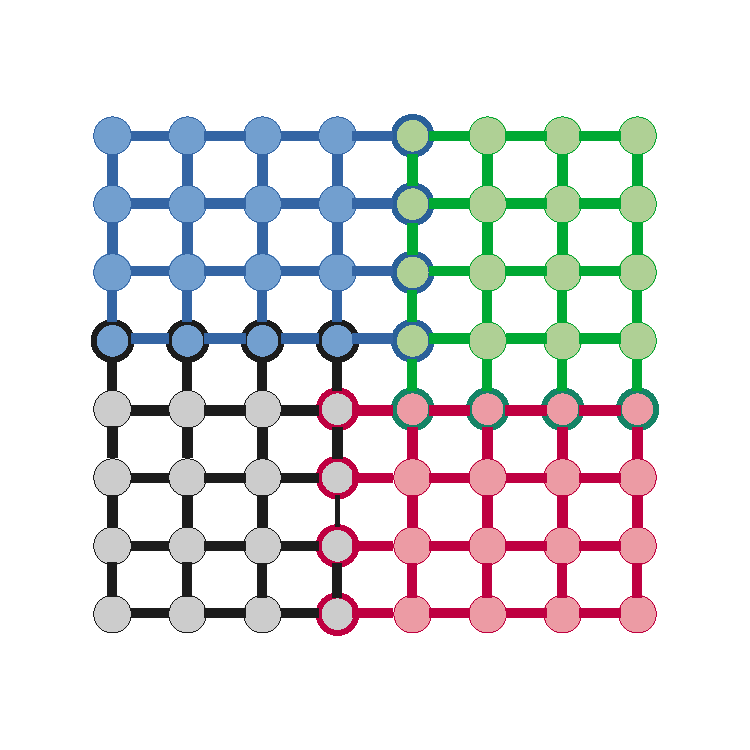
\includegraphics[width=0.5\linewidth]{images/lattice.pdf}
    \caption{Division of a Square Lattice into 4 subsections as in Lemma \ref{lem:lattice}}. Each corresponds to a sum in the Lindbladian. Highlighted are qudits used to `glue' each sublattice to its clockwise neighbor.
    \label{fig:lattice}
\end{figure}

\begin{lemma} \label{lem:lattice} \normalfont
     Consider a square lattice graph $G$ in spatial dimension $D > 1$ of side length $x$, so the total number of qudits is $x^D$. Let $\L = \sum_{(v, w) \in G} \L_{v,w}$ be a Lindbladian that applies parallel, random 2-qudit interactions on edges of $G$. Subdivide the lattice into $2^D$ sublattices each of $x/2$ qudits, where corners join at the center. For each $r \in 1 \dots 2^D$, let the Lindbladian $\L_r$ be that including each of the terms in the $r$th sublattice, as well as the terms joining it to the next sublattice on a contiguous path. Assume these Lindbladians obey the gluing Assumption \ref{assump:glue} with constants $c$ and $q$. If each $\L_r$ has $\lambda$-CMLSI, then $\L$ has $\beta_{\epsilon}^{2^D-1} \lambda$-CMLSI with $\epsilon \leq c / \exp_q((x/2)^{D-1})$.
\end{lemma}
\begin{proof}
    Let $\L[1, s] := \L_1 + \dots + \L_s$. Using Lemma \ref{lem:combine}, if $\L[1,s]$ and $\L_{s+1}$ have $\lambda_s$-CMLSI, then $\L[1, s+1]$ has $\lambda_{s+1}$-CMLSI with $\lambda_{s+1} = \beta_\epsilon \lambda_s$ with $\epsilon \leq c / \exp_q((x/2)^{D-1})$. This essentially yields a recurrence relation. After $2^D-1$ gluings, $\L$ has $\beta_{\epsilon}^{2^D-1} \lambda$-CMLSI.
\end{proof}
\begin{theorem}
    Consider a square lattice graph $G$ in spatial dimension $D > 1$ of side length $x$, so the total number of qudits is $x^D$. Let $\L = \sum_{(v, w) \in G} \L_{v,w}$ be a Lindbladian that applies parallel, random 2-qudit interactions on edges of $G$. Assume that the gluing assumption holds with constants $c$ and $q$ for sublattice Lindbladians potentially including boundaries. For any $\delta \in (0,1)$, if sub-blocks of size at most $2 \lceil \log_q (3 b c q ( 2^{D} - 1 ) / \delta) / (D-1) \rceil $ have $\lambda$-CMLSI, then $\L$ has $\lambda \times (1-\delta)$-CMLSI.
\end{theorem}
\begin{proof}
    Given a target error $\delta > 0$, fix a minimum block size $m$ that we will assume to be a power of 2 and choose explicitly later. The next step is then to apply Lemma \ref{lem:lattice} recursively until the lattice is divided into blocks of size $m$, yielding that
    \begin{equation}
        \lambda_{\L} \geq \lambda \times \prod_{\ell = \log_2 m}^{\log_2 x} \beta[c \exp_q(- 2^{(\ell-1)(D-1)})]^{2^D - 1} \pl.
    \end{equation}
    Using Bernoulli's inequality with the assumption that $\beta_\epsilon \geq 1 - b \epsilon$,
    \begin{equation}
    \begin{split}
        \lambda_{\L} & \geq \lambda \times \bigg ( 1 - b c \big ( 2^{D} - 1 \big ) \sum_{\ell = \log_2 m}^{\log_2 x} \exp_q(- 2^{(\ell-1)(D-1)}) \bigg ) \pl.
        \\ & = \lambda \times \bigg ( 1 - b c \big ( 2^{D} - 1 \big )  \sum_{\ell = 0}^{\log_2 (x/m)} \exp_q(-  m^{D-1} \times 2^{(D-1) \ell} / 2) \bigg ) \pl.
        \\ & = \lambda \times \bigg ( 1 - b c \big ( 2^{D} - 1 \big ) \exp_q (- m^{D-1}) \sum_{\ell = 0}^{\log_2 (x/m)} \exp_q(- 2^{(D-1) \ell} / 2) \bigg ) \pl.
    \end{split}
    \end{equation}
    Subsequent terms in the series shrink much faster than geometrically. Therefore, an upper bound is that
    \begin{equation}
        \sum_{\ell = 0}^{\log_2 (x/m)} \exp_q(- 2^{(D-1) \ell} / 2) \leq \frac{1}{1-1/\sqrt{q}} = \frac{\sqrt{q}}{\sqrt{q}-1} \leq 3 q \pl,
    \end{equation}
    where the last inequality follows that $q \geq 2$. Therefore,
    \begin{equation}
        \lambda_{\L} \geq \lambda \times \bigg ( 1 - 3 b c q \big ( 2^{D} - 1 \big ) \exp_q (- m^{D-1}) \bigg ) \pl.
    \end{equation}
    For error tolerance $\delta$ it suffices that $m \geq \log_q (3 b c q ( 2^{D} - 1 ) / \delta) / (D-1)$. Therefore, we may set $m$ to be the smallest power of 2 that achieves this, which is not bigger than $2 \lceil \log_q (3 b c q ( 2^{D} - 1 ) / \delta) / (D-1) \rceil $.
\end{proof}

{\color{blue} This would appear also to hold for random gate channels, unsurprisingly - again might be able to convert between this and the Lindbladian picture. More surprisingly, it would also seem to hold for particular \textbf{fixed architectures} on these lattices. Would need to check that.

Does the gluing Lemma already give a better result for these lattice architectures with relative error convergence? It can't, because once we go below logarithmic size, should run into error buildup. Also would violate no-go theorems for random circuits. Should explain these subtleties.

Is there a no-go Theorem for 1-D brickwork? Here we would see some bottlenecking involving the gluing lemma, although the nearly optimal earlier results suggest the $n$-dependence is at least extremely weak.}

\section{Fermions}
What do we need for the above strategies to yield decay for fermions?
\begin{enumerate}
    \item We need some sort of gluing. Ideally, maybe we would find that if $\L_1$ and $\L_2$ are two Lindbladians made of fermionic terms (whatever that particular form is), and they share $m$ fermions, then $m$ is the elementary unit number in gluing. Less ideally, we could probably work with a situation in which $m$ is the number of actual terms shared by $\L_1$ and $\L_2$.
    \item 
\end{enumerate}
\color{blue}
\subsection{2-fold Commutativity Problem?}
Consider a channel of the form
\begin{equation}
    \Phi(\rho) = \sum_S p_S \bigg ( \prod_{j \in S} \psi_j \bigg)^{\otimes k} \rho \bigg ( \prod_{j \in S} \psi_j \bigg)^{\dagger \otimes k} \pl,
\end{equation}
where each $\psi_j$ is a fermion, each $S$ is some sequence of indices, and $p_S$ is the probability weighting sequence $S$. Now consider two such sequences, $S$ and $S'$. When $k = 2$, it would appear that
\begin{equation}
    \bigg [ \bigg ( \prod_{j \in S} \psi_j \bigg)^{\otimes 2}, \bigg ( \prod_{i \in S'} \psi_i \bigg )^{\otimes 2} \bigg ] = 0 \pl.
\end{equation}
This follows from the observation that the original sequences would either commute (if they share an even number of fermions, including 0) or anticommute (if they share an odd number of fermions). But when $k = 2$, if the sequences anticommute, then the signs cancel. Hence it would seem that for $k=2$, all such unitary conjugations commute. \textbf{Does this refute that channels of this form, including those arising from semigroups at finite time, can form 2-design twirls? Does this barrier apply to (Brownian) SYK?}

The problem would be that the algebra generated by 2-fold fermion strings is commutative, so it contains itself in its commutant. This would be expected to store $O(n)$ (classical) bits of information in an $n$-fermion system. In contrast, the commutant of the group $\{u^{\otimes 2} : u \in U(d) \}$ in dimension $d$ stores essentially 1 bit of information, corresponding to whether a state is in the symmetric or antisymmetric subspace.
